\documentclass[a4paper,final]{report}
\usepackage[14pt]{extsizes}
\pagestyle{plain}
\usepackage[T2A]{fontenc}
\usepackage[utf8]{inputenc}
\usepackage[russian,english]{babel}
\usepackage[pdftex]{hyperref}
\usepackage[left=3cm, right=1cm, vmargin=2cm]{geometry}
\hbadness=999999 
\usepackage{hypcap}

\usepackage{mathtext} 
\usepackage{placeins}
\usepackage{indentfirst} 
\frenchspacing

\usepackage{enumitem}

\usepackage{titletoc}
\usepackage{setspace}
\sloppy
\usepackage{titlesec}
\titlespacing\section{1.25cm}{0cm}{12pt}
\titlespacing\subsection{1.25cm}{0cm}{12pt}

\usepackage{tocloft}
\setlength{\cftbeforetoctitleskip}{-4em}
\setlist{nosep,wide}
\setlength{\topsep}{-20pt}
\setenumerate[1]{label=\arabic*.}

\usepackage{multicol}
\usepackage{multirow}

\usepackage[final]{graphicx}

\usepackage[tableposition=top,singlelinecheck=false,hypcap=true]{caption}
\usepackage{subcaption}
\DeclareCaptionLabelFormat{gostfigure}{Рис. #2}
\DeclareCaptionLabelFormat{gosttable}{Таблица #2}
\renewcommand{\labelenumii}{\arabic{enumi}.\arabic{enumii}.} 
\DeclareCaptionLabelSeparator{gost}{~---~}
\captionsetup{labelsep=gost}
\captionsetup*[table]{labelformat=gosttable, margin={1.25cm,0pt}}
\captionsetup*[figure]{labelformat=gostfigure,justification=centering}
\renewcommand{\thesubfigure}{\asbuk{subfigure}}

\usepackage[final]{listings}
\usepackage{xcolor}
\usepackage{caption}

\lstset{
	language=C++,                 
	basicstyle=\footnotesize, 
	numbers=left,     
	numberstyle=\tiny,       
	stepnumber=1,          
	firstnumber=1,
	numberfirstline=true
	numbersep=5pt, 
	identifierstyle=\color{gray},
	keywordstyle=\color{blue}\bfseries,
	commentstyle=\color{green},      
	stringstyle=\color{red},   
	morecomment=[l][\color{pink}]{\#},
	showspaces=false,           
	showstringspaces=false,      
	showtabs=false,             
	tabsize=4,                
	captionpos=t,              
	breaklines=true,           
	breakatwhitespace=false,
	extendedchars=true,
	frame=tb,
	title=\lstname
}


\begin{document}
	%--------------------------------------------------------------------------------
	%	ТИТУЛЬНЫЙ ЛИСТ
	%--------------------------------------------------------------------------------
	\begin{titlepage}
	
		\begin{center} 
			\MakeUppercase{Министерство образования и науки Российской федерации} \linebreak  
			\MakeUppercase{Федеральное государственное автономное образовательное учреждение} \linebreak
			«Нижегородский государственный университет им. Н.И. Лобачевского\\[0.2cm] 
			Национальный исследовательский университет\\[0.1cm] 
			Институт информационных технологий, математики и механики \\[0.1cm]  
			Кафедра математического обеспечения и суперкомпьютерных технологий\\[2.5cm]
			{\huge \bfseries Отчет \\[0.1cm]
				\Large \mdseries по лабораторной работе \\[0,1cm]
				\Large \mdseries по дисциплине «Параллельное программирование» \\[1cm]
				\Large \bfseries Поразрядная сортировка для целых чисел с чётно-нечётным слиянием Бэтчера}\\[3cm]
		\end{center}
    
		\begin{flushright} \large
			{Проверил} \\[0.1cm]
			{кандидат технических наук, доцент}\\[0.1cm]
			{\underline{\hspace{2,35in}} Сысоев А.В.}\\[0.1cm]
			{<<\underline{\hspace{0,25in}}>>\underline{\hspace{2,55in}}20\underline{\hspace{0,3in}}г.} \\[0.1cm]
			{Выполнил} \\[0.1cm]
			{студент группы 381706-2} \\[0.1cm]
			{\underline{\hspace{2,1in}} Хрулева А.А.} \\[0.1cm]
			{<<\underline{\hspace{0,25in}}>>\underline{\hspace{2,55in}}20\underline{\hspace{0,3in}}г.} \\[3cm]
		\end{flushright}
		
		\centering{
			Нижний Новгород\\
			\the\year { г.}
		}
	\end{titlepage}
	
	%--------------------------------------------------------------------------------
	%	АВТОМАТИЧЕСКИ СОБИРАЕМОЕ СОДЕРЖАНИЕ
	%--------------------------------------------------------------------------------
	\begin{spacing}{1.5}  
		\renewcommand{\contentsname}{\centerline{\Large{Cодержание}}}
		\dottedcontents{chapter}[1.6em]{}{1.6em}{1pc}
		\tableofcontents
		\setcounter{page}{2}
		
		\newpage
		%--------------------------------------------------------------------------------
		%	ВВЕДЕНИЕ
		%--------------------------------------------------------------------------------
		\section*{\centering Введение}
		\addcontentsline{toc}{section}{Введение}

		
		\setlength{\parindent}{1.25cm}
		\setlength{\parskip}{8pt}
		
        \par
        В 21 веке сложность компьютерных задач, а так же вычислительная мощность и потребность в сортируемости больших объёмов данных значительно возрасла. Одним из самых востребованных алгоритмов на сегодняшний день является алгоритм сортировки. Существует множество разных сортировок, под различные задачи с различными ограничениями, например: поразрядная сортировка, сортировка Хоара, сортировка Шелла. В настоящее время найти самый быстросортируемый алгоритм является одной из важнейших задач программирования, который уменьшает время работы программы и увеличивает её эффективность. Чтобы учучшить второй пункт используем параллельные технологии и библиотеки, такие как: открытый стандарт OpenMP, библиотеки шаблонов С++ от Intel - Intel Threading Building Blocks.
        В этом отчёте представлены данные нескольких лабораборных работ, основанных на алгоритме поразрядной сортировки с чётно-нечётным слиянием Бэтчера. Алгоритм покажет, как примененение технологий распараллеливания увеличивает эффективность всеё программы.
		
		\newpage
		%--------------------------------------------------------------------------------
		%	ПОСТАНОВКА ЗАДАЧИ 
		%--------------------------------------------------------------------------------
		
		\renewcommand*{\thesection}{\arabic{section}}
		\section{Постановка задачи}
		
		\par В лабораторной работе нам необходимо проверить и изучить эффективность алгоритма поразрядной сортировки с чётно-нечётным слиянием Бэтчера на параллельных OpenMP и Intel TBB технологиях. 
		Соответсвенно ход работы у нас будет выглядеть как:
		\begin{itemize} 
			\item[--] написать последовательную версию алгоритма;
			\item[--] написать параллельную версию алгоритма на технологии OpenMP;
			\item[--] написать параллельную версию алгоритма на технологии Intel TBB;
			\item[--] изучить эффективность аллгоритма на разных объёмах массивов;
			\item[--] провести анализ эффективности времени работы технологий относительно друг друга и последовательной версии алгоритма, учитывая объёмы данных, колличество потоков и характеристик компьютера.
		\end{itemize}
		
		\newpage
		
		%--------------------------------------------------------------------------------
		%	ОПИСАНИЕ АЛГОРИТМА 
		%--------------------------------------------------------------------------------
		\section{Описание алгоритма}
		
		\par Поразрядная сортировка относится к быстрым, но ограниченным алгоритмам(не универсальная сортировка, работает только с целыми числами). Основнаяя её идея - это сортировка подсчётом.
		\par Поразрядная сортировка имеет две модификации: 
		\begin{itemize} 
			\item[--] Most Significant Digit, MSD (Нисходящая поразрядная сортировка, от старшего разряда к младшему); 
			\item[--] Least Significant Digit. LSD (Восходящая поразрядная сортировка, от младшего разряда к старшему); 
		\end{itemize}
		В данной работе был применен алгоритм LSD как наиболее эффективный (и подходящий). 
		\par Идея поразрядной восходящей сортировки (Least Significant Digit (LSD) Radix Sort) заключается в том, что выполняется последовательная сортировка чисел по разрядам (от младшего разряда к старшему).
		\par Эффективность алгоритма O(k * (N + m)), где k – число разрядов, N – число элементов, m – число возможных значений (число элементов системы счисления).Т.е. эффективность при правильно реализованном алгоритме линейная.
		\par Общая идея алгоритма быстрой сортировки состоит в следующем: 
		\begin{itemize} 
			\item[--] На первой итерации сортировки выполняется размещение элементов в отсортированном порядке по младшему разряду чисел;
			\item[--] На следующей итерации сортируются элементы по второму разряду;
			\item[--] Далее выполняется упорядочивание элементов по третьему разряду;
			\item[--] -//-;
			\item[--] На последнем шаге выполняется сортировка по старшему разряду ;
		\end{itemize}
		
		\par Для увеличения эффективности работы алгоритма входные данные представлены в виде битовых чисел. 
		\vspace{2ex}
		\par \textbf{Разбиение «Четно-нечетное слияние Бэтчера»}
		\par Чётно-нечётное слияние Бэтчера заключается в том, что два упорядоченных массива, которые необходимо слить, разделяются на чётные и нечётные элементы. Такое слияние может быть выполнено параллельно. 
		\par Чтобы массив стал окончательно отсортированным, достаточно сравнить пары элементов, стоящие на нечётной и чётной позициях. Первый и последний элементы массива проверять не надо, т.к. они являются минимальным и максимальным элементов массивов. 
		\par Чётно-нечётное слияние Бэтчера позволяет задействовать 2 потока при слиянии двух упорядоченных массивов. В этом случае слияние N массивов могут выполнять N параллельных потоков. На следующем шаге слияние N/2 полученных массивов будут выполнять N/2 потоков и т.д. На последнем шаге два массива будут сливать 2 потока 
 
        \vspace{2ex}
        
		\begin{center}
        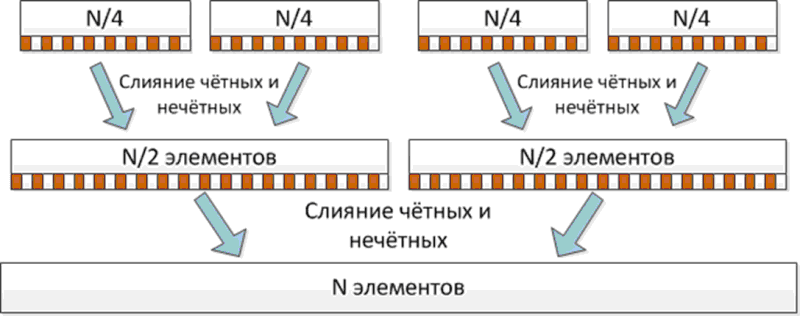
\includegraphics[width=\linewidth]{../../../../modules/reports/khruleva_a_radix_batcher_sort/ph1.png}
        \captionof{figure}{Чётно-нечётное слияние Бэтчера}
        \end{center}
        
		\newpage
		%--------------------------------------------------------------------------------
		%	ОПИСАНИЕ СХЕМЫ РАСПАРАЛЛЕЛИВАНИЯ
		%--------------------------------------------------------------------------------
		\section{Описание схемы распараллеливания}
		
		\par Реализованные OpenMP и TBB версии имеют одинаковую структуру, поэтому их можно представить в виде одной схемы: 
		\vspace{2ex}
        
		\begin{center}
        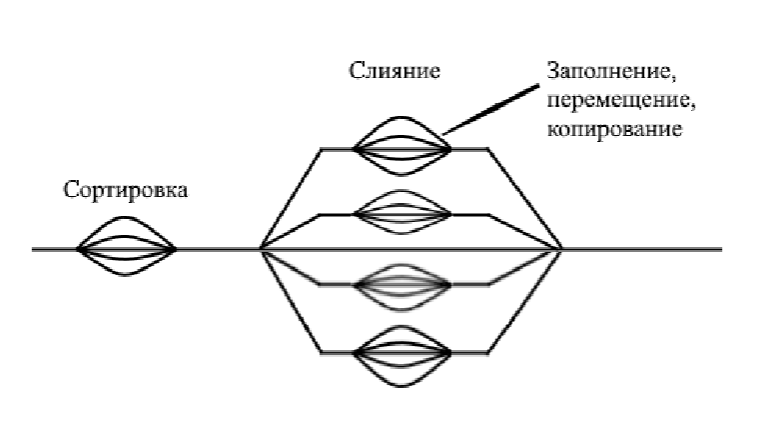
\includegraphics[width=\linewidth]{../../../../modules/reports/khruleva_a_radix_batcher_sort/ph2.png}
        \captionof{figure}{Схема распараллеливания}
        \end{center}
        
		\vspace{2ex}
        
		\par На этапе «сортировка» в OpenMP сразу массив делится на куски в количестве равном количеству потоков, в TBB при создании дочерних «заданий» когда размер «подмассива» соответствует необходимому разделению на потоки и в обоих случаях «подмассивы» сортируются последовательной версией сортировки (sequentially). После этой части весь массив элементов состоит из отсортированных кусков-«подмассивов».  
		\par На участке «слияние» происходит соответственное последовательное слияние подмассивов (1-2,3-4, и т.д.).   
		\par «Слияние» в данном случае подразумевает слияние четных и нечетных элементов подмассивов отдельно и их соответственное (четно-нечетное) слияние. 
		
		\par Схема слияния: 
			\vspace{2ex}
        
		\begin{center}
        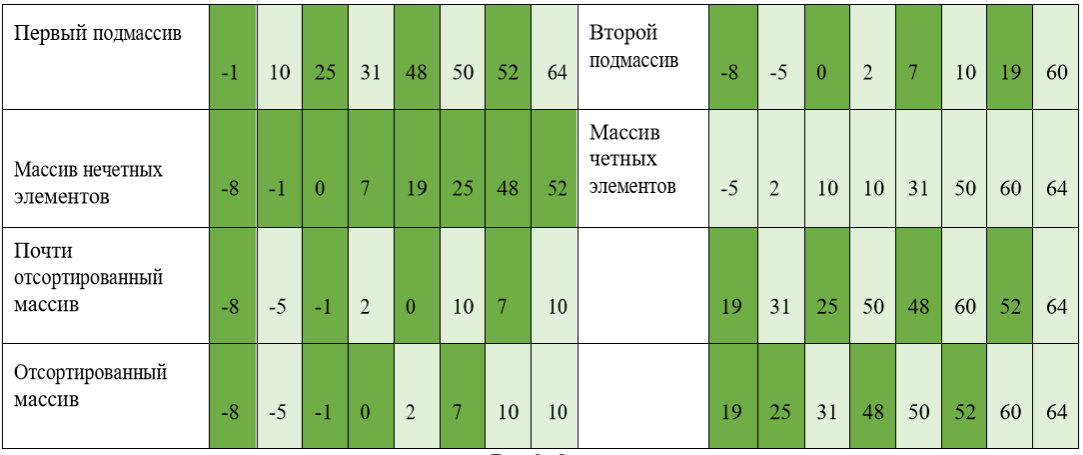
\includegraphics[width=\linewidth]{../../../../modules/reports/khruleva_a_radix_batcher_sort/ph3.png}
        \captionof{figure}{Схема слияния}
        \end{center}
        
		\vspace{2ex}
		
		\newpage
		%--------------------------------------------------------------------------------
		%	ОПИСАНИЕ ПРОГРАММНОЙ РЕАЛИЗАЦИИ
		%--------------------------------------------------------------------------------
		\begin{spacing} {0.5}
			\section{Описание программной реализации}
		\end{spacing}
		\subsection{Описание OpemMP версии}
		
		\par  Реализация поразрядной сортировки для целых чисел с четно- нечетным слиянием Бэтчера с использованием средств OpenMP (radix\_batcher\_sort.cpp и main.cpp) 
		\par  Вызываемая функция сортировки называется  least\_significant\_digit\_sort, в которой первый параметр int* arr – сортируемый вектор, второй int size – размер сортируемого вектора, третий  int bits– битовое представление. 
		\begin{spacing}{0}
\end{spacing}

\begin{lstlisting}[language=C++]
void love_sex_dream_sort(int * arr, int size, int bits=BITS)
{
  int ** numbers = new int*[2];
  numbers[0] = new int[size];
  numbers[1] = new int[size];
  int counters[] = {0, 0};

  for (int bit_num = 0; bit_num < bits; ++bit_num)
  {
    for (int i = 0; i < size; ++i)
    {
      int bit = ((arr[i] >> bit_num) & 1);
      numbers[bit][counters[bit]] = arr[i];
      ++counters[bit];
    }
    int k = 0;
    for (int i = 0; i < counters[0]; ++i, ++k)
      arr[k] = numbers[0][i];
    for (int i = 0; i < counters[1]; ++i, ++k)
      arr[k] = numbers[1][i];

    counters[0] = counters[1] = 0;
  }

  delete[] numbers[0];
  delete[] numbers[1];
  delete[] numbers;
}
// Parallel OpenMP Radix sort }
\end{lstlisting}
		\par Общая структура:Имеется k процессов, Исходный массив делится на k подмассивов длиной, кратной 2 (то есть длина исходного массива должна быть кратна 2k),каждый подмассив сортируется lsd,далее для каждой пары соседних подмассивов параллельно запускаются параллельный,алгоритм слияния odd-even merge. Внутри слияния делаем все по Рис.3.
				\begin{spacing}{0}
\end{spacing}

\begin{lstlisting}[language=C++]
void odd_even_merger(int * arr, int size)
{
  int half_size = size >> 1; 

  int * left_arr = new int[half_size];
  int * right_arr = new int[half_size];

  #pragma omp parallel num_threads(2)
  {
    #pragma omp single nowait
    {
      odd_even_simple_merge(arr, size, left_arr);
    }

    #pragma omp single nowait
    {
      odd_even_simple_merge(arr + 1, size, right_arr);
    }

    #pragma omp barrier
  }

/*
  parallel for

1: 0 1 2 3
2: 4 5 6 7
... half_size-1

*/
  #pragma omp parallel for
  for (int i = 0; i < half_size; ++i)
  {
    if (left_arr[i] < right_arr[i])
    {
      arr[2 * i] = left_arr[i];
      arr[2 * i + 1] = right_arr[i];
    }
    else
    {
      arr[2 * i] = right_arr[i];
      arr[2 * i + 1] = left_arr[i];
    }
  }


  #pragma omp parallel for
  for(int i = 0; i < size - 1; ++i)
    compare_exchange(arr + i, arr + i + 1);

  delete[] left_arr;
  delete[] right_arr;
}

// Parallel OpenMP Merge }
\end{lstlisting}
		\par  Алгоритм сделан так чтобы получилось максимальное ускорение, поэтому массив будет представлен в битовом виде. Последовательная версия используется из Seq.cpp(см. в приложении)
		
		
		\par Функция void odd\_even\_merger используется для  слияния массивов четных и нечетных элементов.
		\par Т.е. аллгоритм сводится к такому описанию: массив разделяется на 2 раные части, которые идут каждая на свой поток, потом каждая из этих частей так же разделяется на 2 части в виде: в одной нечётные эллементы, в другой чётные. Получается массив разделённый на 4 части. Далее сливаются нечётные части с нечётными, а чётные с чётными обычным слиянием, получается 2 отсортированных массива. Далее чётно-нечётно сливаем и ещё раз проходимся по массиву lsd для полной уверенности, что массив отсортирован.
			\begin{spacing}{0}
\end{spacing}

\begin{lstlisting}[language=C++]
		/*
5 2 1 3    8 18 0 257

thread1:
lsd(5 2 1 3)

thread2:
lsd(8 18 0 257)


arr + 1

1 2 3 5   0 8 18 257

thread 1:
1 3    0 18  simple merge -->   0 1 3 18

thread 2:
2 5    8 257  simple merge -->   2 5 8 257


   thread: 1 1  2 2   3 3
        i: 0 1  2 3   4 5
 left_arr: 0 1  2 7   8 9
right_arr: 1 1  2 3   4 10

0 1 2 3   4 5 6 7   8 9 10 11
  1     1      2      2
0  1  1  1   2   2  3   7   4 8  9 10
     1     1       2

1 100  n
2 50   n/2
4 25   n/4


          1      2     3      4
result = 0  2  1  5  3  8  18  257
             1     2     3
*/
	// Parallel OpenMP algorithm }
\end{lstlisting}	
		\subsection{Описание TBB версии}
		
		\par Реализация поразрядной сортировки для целых чисел с четно- нечетным слиянием Бэтчера с использованием средств TBB (ParallelTBB.cpp см. в приложении) 
		\par Вызываемая функция сортировки называется void Start\_TBB\_Sorting(int *arr, int size, int threads), в которой первый параметр – сортируемый массив, второй –  размер сортируемого массива, третий – количество потоков.  Общая структура: Запускаем корневое задание, которое, по сути, рекурсивно вызовет столько дочерних задний сколько есть потоков и когда заданная порция (которая зависит от кол-ва потоков) будет больше числа элементов в подмассиве запустится последовательная версия сортировки из solver. Далее созданные задания также, по сути, делают слияния аналогично пункту из OpenMP.
		\par Класс используемый в работе class SortingBody необходим для запуска самого тела сортировки: таких же заданий для следующих уровней, выделения массивов четных и нечетных элементов и их распределения в массив, а также запуск последовательной сортировки для кусков необходимого размера.
		
		\par В алгоритме используется функция-конвертер которая преобразует массив в вектор и наоборот. Она необходима т.к. получилось реализовать программу только используя массив, а Solution.h версия рассчитана на вектор. 
		\par Последовательная версия используется из Solution.h.h
		\par Класс используемый в работе class SortingBody необходим для запуска самого тела сортировки: таких же заданий для следующих уровней, выделения массивов четных и нечетных элементов и их распределения в массив, а также запуск последовательной сортировки для кусков необходимого размера. 
 . \begin{spacing}{0}
\end{spacing}

\begin{lstlisting}[language=C++]

class SortingBody : public task
{ 
private:  
int *arr;  
int size;  
int portion; 
 
public:  SortingBody(int *_arr, int _size, int _portion) : arr(_arr), size(_size), portion(_portion)
{} 
 
 task* execute()  
 {  
        if (size <= portion)   
        {    
             transformed_sort(arr, size);   
        }   
        else   
        {    
          int s = size / 2;    
          SortingBody &sorter_one = *new (allocate_child()) SortingBody(arr, s, portion);   
          SortingBody &sorter_two = *new (allocate_child()) SortingBody(arr + s, size - s, portion);    
          set_ref_count(3);    
          spawn(sorter_one);    
          spawn_and_wait_for_all(sorter_two);    
          EvenSelector &evenSelector = *new (allocate_child()) EvenSelector(arr, s, size - s);    
          OddSelector &oddSelector = *new (allocate_child()) OddSelector(arr, s, size - s);    
          set_ref_count(3);   
          spawn(evenSelector);    
          spawn_and_wait_for_all(oddSelector); 
           parallel_for(blocked_range<int>(1, size), Comparator(arr));   
           }   return NULL;
        } 
    }; 
   
// Parallel TBB SortingBody }
\end{lstlisting} 
		\par Классы class OddSelector и class EvenSelector каждый из которых выбирает из массивов нечетные и четные элементы соответственно в упорядоченном виде и сразу же распределяет их по нечетным и четным местам массива соответственно (код см. в приложении).
		\par Функция void transformed\_sort(int* arr, int size) производящая конвертирование и сортировку последовательной версией (код см. в приложении).
		\par Класс class Comparator необходимый для пробега по массиву и проверки что массив отсортирован, если соседние элементы стоят неправильно он их обменивает 
		
		\newpage
		%--------------------------------------------------------------------------------
		%	РЕЗУЛЬТАТЫ ЭКСПЕРИМЕНТОВ, ОПИСАНИЕ ПОДТВЕРЖДЕНИЯ КОРРЕКТНОСТИ
		%--------------------------------------------------------------------------------
		\section{Результаты экспериментов}
		
		\par Эксперименты проводятся на компьютере со следующими характеристиками: процессор	Intel(R) Core(TM) i5-8250U CPU $@$ 1.60GHz, 2400 MGz ядер: 4, логических процессоров: 8, установленная оперативная память (RAM) - 8,00 ГБ, кэш L1 - 256 КБ, кэш L2 - 1 МБ, кэш L3 - 6,0 МБ. 
		\par Сортировка проводилась для массивов размерами: 
              1) 100000; 2) 1000000; 3) 10000000; 
		\par элементов для последовательной версии, параллельной версии OMP и параллельной версии TBB для: 
        1) 1 потока; 2) 2 потоков; 3) 4 потоков; 4) 8 потоков. 
        \par Результаты работы представляется в виде значения времени работы сортировки и сравнивались по отношению со временем работы последовательной версии при соответствующих значениях размера массива, а так же внутри самой параллельной версии относительно времени работы при различных значениях количества потоков. 
			\begin{table}[ht!]
			\caption{Ускорения OpenMP и TBB версий}
			\centering
			\begin{tabular}{|p{2.2cm}|p{2.4cm}|p{2.5cm}|p{2.6cm}|p{2.6cm}|p{2.1cm}|}
				\hline
				
				Кол\-во эл\-ов n & Serial version, s & OpenMP version 2 threads, s & OpenMP version 4 threads,s & OpenMP version 8 threads, s & TBB version 4 threads, s \\ \hline
				
		        100000 & 0,0012851 & 0,0008552 & 0,0007125 & 0,0007916 & 0,0007199 \\ \hline
				
		        1000000 & 0,0121459 & 0,0081467 & 0,0067820 & 0,0069212 & 0,0061776 \\ \hline
				
	        	10000000 & 0,1310553 & 0,0840191 & 0,0721147 & 0,0719626 & 0,0621048 \\ \hline
	        	
				100000000 & 1,6234433 & 1,0196194 & 0,8693612 & 0,6792818 & 0,8532456 \\ \hline
				
			\end{tabular}
		\end{table}
		
		\begin{table}[ht!]
			\caption{Ускорения OpenMP и TBB версий}
			\centering
			\begin{tabular}{|p{2.8cm}|p{3.1cm}|p{3.1cm}|p{3.1cm}|p{2.8cm}|}
				\hline
				
					Кол-во эл-ов, n & Ser/OpenMP 2  & Ser/OpenMP 4 & Ser/OpenMP 8 & Ser/TBB  \\ \hline
				
				100000 & 1,506677 & 1,808435 & 1,623421 & 1,7851091 \\ \hline
				
				1000000 & 1,490899 & 1,790902 & 1,754884 & 1,9661195 \\ \hline
				
				10000000 & 1,559827 & 1,817317 & 1,821158 & 2,110228 \\ \hline
				
				100000000 & 1,592205 & 1,867398 & 2,389941 & 1,9026682 \\ \hline
				
			\end{tabular}
		\end{table}
		
		\vspace{4ex}
        
		\begin{center}
        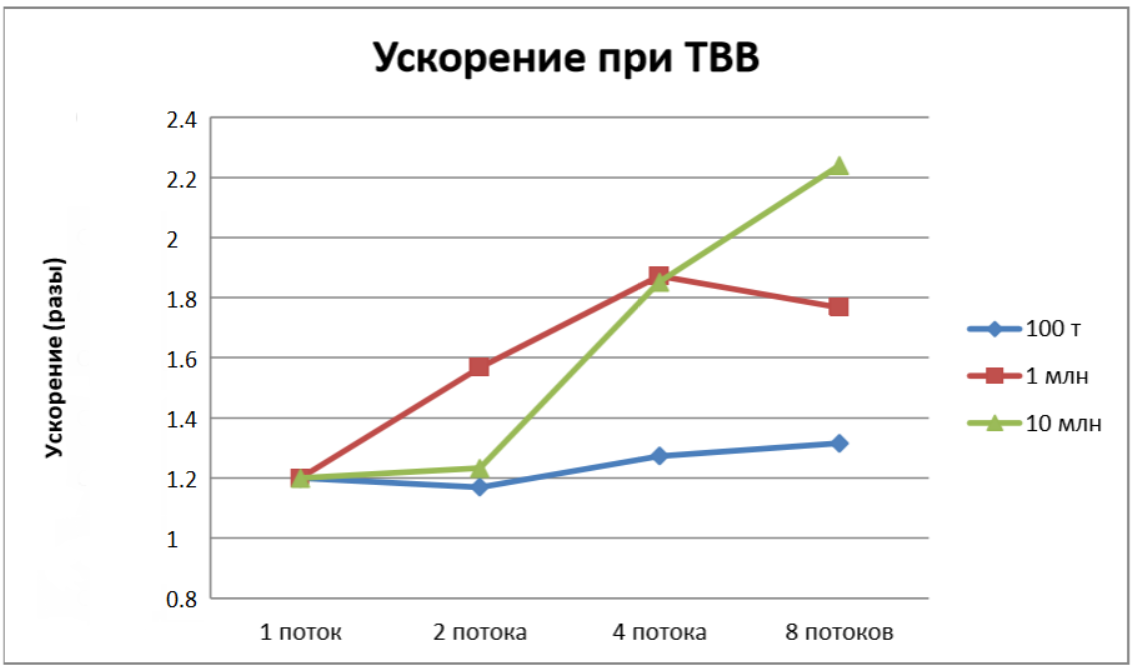
\includegraphics[width=\linewidth]{../../../../modules/reports/khruleva_a_radix_batcher_sort/ph4.png}
        \captionof{figure}{График ускорения TBB на потоках}
        \end{center}
        
		\vspace{2ex}
		
		
		\newpage
		%--------------------------------------------------------------------------------
		%	ВЫВОДЫ ИЗ РЕЗУЛЬТАТОВ ЭКСПЕРИМЕНТОВ
		%--------------------------------------------------------------------------------
		\section{Выводы из результатов экспериментов}
		
		\parВ ходе работы была реализована Поразрядная сортировка для целых чисел с четно-нечетным слиянием Бэтчера в последовательной и 2-х параллельных версиях, изучены и опробованы такие средства параллельной разработки как Open Multi-Processing(OpenMP) и Intel Threading Building Blocks(TBB). 
		\par По самой сортировке видно, что ее эффективность вполне соответствует теоретическим ожиданиям, а также видно, что сама последовательная сортировка (Восходящая поразрядная, LSD) очень устойчивая и генерация исходных данных массивов не влияют на результат (нет худшего случая при случайном распределении данных)
		\par Масштабируемость по данным: 
		\par Сложно оценить, т.к. не хватает данных, и при текущих условиях сложно более глубоко проверить масштабируемость. По текущим же данным при росте размера массива ускорение остается в целом стабильным. 
		\par Масштабируемость по потокам: 
		\par По результатам эксперимента видно, что при увеличении числа потоков для данной задачи, до 4 ускорение алгоритма быстро растет, при увеличении до 8 либо немного падает, либо остается на том же уровне. Скорее всего причина в том, как именно аппаратная часть реализует работу при восьми потоках на 4 ядрах. 
		\par у OpenMP наблюдается отсутствие сильной зависимости от размера массива (возможно дело в ограничениях «железа» или в «малом» количестве элементов). Однако, в целом само поведение ускорения здесь более спокойное чем на следующем графике работы TBB. Оптимальным количеством потоков для наилучших показателей ускорения у OpenMP в среднем является 4 потока(, причина может быть, в аппаратных составляющих (4-х ядерный процессор). Хорошо прослеживается тенденция увеличения ускорения при увеличении количества потоков в 2 раза от последовательного исполнения, но приближаясь к значению 4-х потоков, ускорение снижается, а при 8 потоках и вовсе становится схожим со значением при 4 потоке. Причиной тому скорее всего является увеличение времени слияния, так как данных дастаточно большое колличесво, для алгоритма сортировки это явное улучшение и сокращение работы, а для алгоритма слияния наоборот.  
        \par У средств TBB похожая ситуация, хотя, здесь отрыв 4 потоков не так очевиден, однако он все же есть, данные для 1,2 и 4 потоков представлены только на графике, так как записывать их в таблицу не было целесообразно. Так же можно заметить, что более высокое ускорение при 4-8 потоках хотя и выдает хорошие результаты, весьма нестабильно и может выдавать как хорошие показатели, так и не очень. В целом же ускорение весьма приличное для проводимого опыта. 
        \par Также интересно выяснить какие из средств параллельного программирования – TBB или OpenMP оказались на высоте в данном алгоритме. Посмотрев на значения таблиц и представления графика сразу становится очевидно, что во всех случаях более высокие показатели у средств TBB, и даже если сравнивать на разных размерах массивов, картина не меняется. И на 2-х, и на 4-х, и на 8-ми потоках TBB более эффективно выполняли сортировку и можно заметить, что при увеличении числа потоков ускорение у TBB становится больше. Это может объясняться  различием в реализации  распараллеливания – у TBB более эффективно – а так же самим видоизменением алгоритма.
		
		\newpage
		%--------------------------------------------------------------------------------
		%	ЗАКЛЮЧЕНИЕ
		%--------------------------------------------------------------------------------
		
		\section*{\centering Заключение}
		\addcontentsline{toc}{section}{Заключение}
		
		\par В результате работы была написана программа (набор программ), позволяющая создавать случайные массивы, сортировать их паразрядно с чётно-нечётным слиянем Бэтчера, как последовательным, так и параллельным алгоритмом (с помощью технологий OpenMP и Intel Threading Building Blocks) , а также вести обработку полученных по ним данных. Для любого количества данных и потоков алгоритм является корректным (корректность оцениваласть на коэффициенте ускорения от 1,49 до 2,3, который показывает правильную работу алгоритма и технологий) . Проведены серии экспериментов показывающие ускорение параллельного алгоритма, достоинства и важность изучения методов параллельных вычислений. 
		
		\newpage
		%--------------------------------------------------------------------------------
		%	СПИСОК ЛИТЕРАТУРЫ
		%--------------------------------------------------------------------------------
		
		\section*{\centering Список литературы}
		\addcontentsline{toc}{section}{Список литературы}
		
		\begin{enumerate} 
		
		    \item Сиднев А.А., Сысоев А.В., Мееров И.Б.  Оптимизация вычислительно трудоемкого программного модуля для архитектуры Intel Xeon Phi. Линейные сортировки. Сиднев А.А., Сысоев А.В., Мееров И.Б. 
		    
			\item Гергель В.П. Современные языки и технологии параллельного программирования / Гергель В.П. - Издательство Московского Университета, 2012. - 408 с.
			
			\item Сиднев А.А., Сысоев А.В., Мееров И.Б. Учебный курс «Технологии параллельного программирования» Лекционные материалы. 
			
			\item Федотов А. Обзор библиотеки Intel TBB / Федотов А. - SSG/DPD/TCAR/Threading Runtimes, 2017 – 79 с.
			
			\item Мееров И.Б. Инструменты параллельного программирования для систем с общей памятью $/$ Мееров И.Б., Сысоев А.В., Сиднев А.А. – Нижегородский государственный университет им. Н.И.Лобачевского, Факультет Вычислительной математики и кибернетики 2009 – 172 с.
			
			\item Вирт Н. Алгоритмы и структуры данных $/$ Вирт Н. - Издательство Мир, 1989, 360 стр.
			
			\item Антонов А.С. Параллельное программирование с использованием технологии OpenMP: Учебное пособие $/$ Антонов А.С. – М.: Изд-во МГУ, 2009. – 77 с. 
			
		\end{enumerate}
		
		\newpage
		%--------------------------------------------------------------------------------
		%	ПРИЛОЖЕНИЕ А. КОД ПРОГРАММЫ
		%--------------------------------------------------------------------------------
		\begin{spacing}{0.5}
			\section*{\centering Приложение А}
			\addcontentsline{toc}{section}{Приложение А}
		\end{spacing}
		\centerline{(обязательное)}
		\centerline{\bfseriesКод программы} 
		\par Исходный код трех лабораторных работ.

\par Первая лабораторная работа «Последовательная версия поразрядной сортировки для целых чисел счётно-нечётным слиянием Бэтчера»
\begin{spacing}{0}
\end{spacing}

\begin{lstlisting}[language=C++]
#pragma once

#include <vector>
#include <queue>

using namespace std;

int get_max(vector<int>& array_for_sort, const int left_border, const int right_border)
{
	int max = abs(array_for_sort[left_border]);
	for (int i = left_border; i <= right_border; i++)
		if (abs(array_for_sort[i]) > max)
			max = abs(array_for_sort[i]);
	return max;
}
void count_sort(vector<int>& array_for_sort, const int left_border, const int right_border, int digit)
{
	vector<int> output(right_border - left_border + 1);
	int count[10] = { 0 };

	for (int i = left_border; i <= right_border; i++)
		count[(abs(array_for_sort[i]) / digit) % 10]++;

	for (int i = 1; i < 10; i++)
		count[i] += count[i - 1];

	for (int i = right_border; i >= left_border; i--)
	{
		output[count[(abs(array_for_sort[i]) / digit) % 10] - 1] = array_for_sort[i];
		count[(abs(array_for_sort[i]) / digit) % 10]--;
	}

	for (int i = left_border; i <= right_border; i++)
		array_for_sort[i] = output[i];
}

void radix_sort_sol(vector<int>& array_for_sort, const int left_border, const int right_border)
{
	auto num_of_numbers = right_border - left_border + 1;
	vector<int> vec_pos;
	vector<int> vec_neg;

	auto num_of_pos_numbers = 0;
	auto num_of_neg_numbers = 0;

	for (size_t i = left_border; i < right_border + 1; ++i)
		if (array_for_sort[i] >= 0)
			num_of_pos_numbers++;

	num_of_neg_numbers = num_of_numbers - num_of_pos_numbers;

	vec_pos.reserve(num_of_pos_numbers);
	vec_neg.reserve(num_of_neg_numbers);
	vector<int> temp = array_for_sort;
	vector<int>::iterator it_chunk_begin, it_chunk_end;
	it_chunk_begin = temp.begin() + left_border;
	it_chunk_end = temp.begin() + left_border + num_of_numbers;
	copy_if(it_chunk_begin, it_chunk_end, back_inserter(vec_pos), [](int i) { return i >= 0; });
	copy_if(it_chunk_begin, it_chunk_end, back_inserter(vec_neg), [](int i) { return i < 0; });

	const int max_elem = get_max(temp, left_border, right_border);
	for (int curr_digit = 1; max_elem / curr_digit > 0; curr_digit *= 10)
		count_sort(vec_pos, 0, num_of_pos_numbers - 1, curr_digit);
	for (int curr_digit = 1; max_elem / curr_digit > 0; curr_digit *= 10)
		count_sort(vec_neg, 0, num_of_neg_numbers - 1, curr_digit);
	reverse(vec_neg.begin(), vec_neg.end());

	for (int i = left_border, j = 0; i < left_border + num_of_neg_numbers; i++, j++)
		array_for_sort[i] = vec_neg[j];
	for (int i = left_border + num_of_neg_numbers, j = 0; i < right_border + 1; i++, j++)
		array_for_sort[i] = vec_pos[j];
}
//  seq.cpp }
\end{lstlisting} 


\par Вторая лабораторная работа «OpenMP версия поразрядной сортировки для целых чисел счётно-нечётным слиянием Бэтчера
\lstinputlisting[language=C++, caption=OpenMP версия. Заголовочный файл]{../../../../modules/task_2/khruleva_a_radix_batcher_sort/radix_batcher_sort.h}
\lstinputlisting[language=C++, caption=OpenMP версия. Cpp файл]{../../../../modules/task_2/khruleva_a_radix_batcher_sort/radix_batcher_sort.cpp}
\lstinputlisting[language=C++, caption=OpenMP версия. Google Tests]{../../../../modules/task_2/khruleva_a_radix_batcher_sort/main.cpp}


\par Третья лабораторная работа «TBB версия поразрядной сортировки для целых чисел счётно-нечётным слиянием Бэтчера»
\begin{spacing}{0}
\end{spacing}

\begin{lstlisting}[language=C++]
#define _CRT_SECURE_NO_WARNINGS

#include "tbb\task_scheduler_init.h"
#include "tbb\parallel_for.h"
#include "tbb\blocked_range.h"
#include "tbb\tbb.h"
#include <iostream>
#include <cstdio>
#include <string>
#include <vector>

using namespace std;
using namespace tbb;

double time_error;
void radix_sort_sol(vector<int>& array_for_sort, const int left_border, const int right_border);

void transformed_sort(int* arr, int size)
{
	tick_count start = tick_count::now();
	vector<int> convert(size);
	for (int i = 0; i < size; i++)
		convert[i] = arr[i];
	tick_count f_st = tick_count::now();
	radix_sort_sol(convert, 0, size - 1);
	tick_count f_fin = tick_count::now();
	for (int i = 0; i < size; i++)
		arr[i] = convert[i];
	tick_count finish = tick_count::now();
	time_error += ((finish - start) - (f_fin - f_st)).seconds();
}

class EvenSelector : public task
{
private:
	int* arr;
	int size1, size2;

public:
	EvenSelector(int* _arr, int _size1, int _size2) : arr(_arr), size1(_size1), size2(_size2) {
	}

	task* execute()
	{
		int* arr2 = arr + size1;

		int num = (size1 + size2 + 1) / 2;
		int* tmp = new int[num];

		int a = 0, b = 0, i = 0;
		while (a < size1 && b < size2) {
			if (arr[a] <= arr2[b])
			{
				tmp[i] = arr[a];
				a += 2;
			}
			else
			{
				tmp[i] = arr2[b];
				b += 2;
			}
			i++;
		}
		if (a >= size1)
			for (int j = b; j < size2; j += 2, i++)
				tmp[i] = arr2[j];
		else
			for (int j = a; j < size1; j += 2, i++)
				tmp[i] = arr[j];
		for (int j = 0; j < num; ++j)
			arr[j * 2] = tmp[j];
		return NULL;
	}
};

class OddSelector : public task
{
private:
	int* arr;
	int size1, size2;

public:
	OddSelector(int* _arr, int _size1, int _size2) : arr(_arr), size1(_size1), size2(_size2) {
	}

	task* execute()
	{
		int* arr2 = arr + size1;

		int num = (size1 + size2) - (size1 + size2 + 1) / 2;
		int* tmp = new int[num];

		int a = 1, b = 1, i = 0;
		while (a < size1 && b < size2) {
			if (arr[a] <= arr2[b])
			{
				tmp[i] = arr[a];
				a += 2;
			}
			else
			{
				tmp[i] = arr2[b];
				b += 2;
			}
			i++;
		}
		if (a >= size1)
			for (int j = b; j < size2; j += 2, i++)
				tmp[i] = arr2[j];
		else
			for (int j = a; j < size1; j += 2, i++)
				tmp[i] = arr[j];

		for (int j = 0; j < num; ++j)
			arr[j * 2 + 1] = tmp[j];
		return NULL;
	}
};

class Comparator
{
private:
	int* arr;
public:
	Comparator(int* _arr) : arr(_arr) {}

	void operator()(const blocked_range<int>& r) const
	{
		int begin = r.begin(), end = r.end();
		for (int i = begin; i < end; i++)
			if (arr[i - 1] > arr[i])
			{
				int tmp = arr[i - 1];
				arr[i - 1] = arr[i];
				arr[i] = tmp;
			}
	}
};

class SortingBody : public task
{
private:
	int* arr;
	int size;
	int portion;

public:
	SortingBody(int* _arr, int _size, int _portion) : arr(_arr), size(_size), portion(_portion) {}

	task* execute()
	{
		if (size <= portion)
		{
			transformed_sort(arr, size);
		}
		else
		{
			int s = size / 2;
			SortingBody& sorter_one = *new (allocate_child()) SortingBody(arr, s, portion);
			SortingBody& sorter_two = *new (allocate_child()) SortingBody(arr + s, size - s, portion);
			set_ref_count(3);
			spawn(sorter_one);
			spawn_and_wait_for_all(sorter_two);
			EvenSelector& evenSelector = *new (allocate_child()) EvenSelector(arr, s, size - s);
			OddSelector& oddSelector = *new (allocate_child()) OddSelector(arr, s, size - s);
			set_ref_count(3);
			spawn(evenSelector);
			spawn_and_wait_for_all(oddSelector);

			parallel_for(blocked_range<int>(1, size), Comparator(arr));
		}
		return NULL;
	}
};

void Start_TBB_Sorting(int* arr, int size, int threads)
{
	int portion = size / threads;

	if (size % threads != 0)
		portion++;

	SortingBody& sorter = *new (task::allocate_root())
		SortingBody(arr, size, portion);
	task::spawn_root_and_wait(sorter);
}

int main(int argc, char* argv[])
{
	if (argc != 4) {
		cout << "Enter the correct parameters:" << endl;
		cout << "1. The name of the source binary file" << endl;
		cout << "2. The name of the output binary file" << endl;
		cout << "3. The number of threads" << endl;
		return 1;
	}

	int size, threads = atoi(argv[3]);
	int* arr;
	double fict_time;
	time_error = 0;

	freopen(argv[1], "rb", stdin);
	fread(&fict_time, sizeof(fict_time), 1, stdin);
	fread(&size, sizeof(size), 1, stdin);

	arr = new int[size];
	fread(arr, sizeof(*arr), size, stdin);
	double time;

	tick_count start_main = tick_count::now();
	Start_TBB_Sorting(arr, size, threads);
	tick_count finish_main = tick_count::now();

	time = (finish_main - start_main).seconds() - time_error;
	printf("TBB sorting time: %f\n", time);

	freopen(argv[2], "wb", stdout);
	fwrite(&time, sizeof(time), 1, stdout);
	fwrite(&size, sizeof(size), 1, stdout);
	fwrite(arr, sizeof(*arr), size, stdout);
	return 0;
}
//  ParallelTBB.cpp }
\end{lstlisting} 
		
		
	\end{spacing}
	
\end{document}